\section{Literature Review}
This section tackles the investigation of components which make up the proposed high level system depicted in figure \ref{fig:hypothesis}.
There exists a variety of different tools available to realize each system.
With the hardware preexisting, most of the design exists in the software domain.
Various software tools and methodologies are considered.

\subsection{Sensors}
Effective data logging of acceleration, altitude, location and speed all begin with the quality of measurements being made.
Smartphones alone provide a wealth of options.
However, external sensors available to the truck operators offer a variety of options.

\subsubsection{Internal Sensors}
Most smartphones come well-equipped with a wide variety of on-board sensors, such as \ac{gps} sensors, accelerometers, gyroscopes, magnetometers and ambient light sensors, among others \cite{majumder2019smartphone}.
As such, they are capable of inferring a wealth of information related to driving patterns.
This includes dangerous driving behavior, for which algorithms have been developed \cite{li2016dangerous}.

While not all smartphones provide a full suite of sensors, a combination of on-board sensors can be used to measure variables of interest.
\begin{itemize}
\item \textbf{Acceleration}\\
Raw accelerometers provide acceleration readings along 3 axes to encompass a three dimensional space.
Tilting or rotating the smartphone will change the axis on which an applied acceleration is detected.
This will happen often in smartphones which aren't securely mounted, or when traversing steep gradients.
The combined applied acceleration (or resultant acceleration $a_{res}$) can be found by combining the component in each direction, with
\begin{equation}\label{eq:acc}
\begin{split}
a_{res} = \sqrt{a_{x}^2 + a_{y}^2 + a_{z}^2},\\
\end{split}
\end{equation}
where $a_{x}, a_{y}, a_{z}$ denote the acceleration components on each axis.\cite{david2020halliday}

Gravity applies a constant acceleration as well, which is not of interest.
Filters that eliminate this constant gravity component can do so by means of highpass filtering, clearing the constant bias.
However, if this acceleration is sustained for several samples (as is often the case when driving), this momentarily constant acceleration is also filtered out.

The most effective means for determining acceleration excluding gravity is to use a combination of sensors in a strategy usually termed \textit{sensor fusion}.\cite{sasiadek2002sensor}
This method makes additional use of magnetometers and gyroscopes to isolate and remove the gravity component.
An Android \ac{api} abstraction makes use of sensor fusion implementing a so-called \textit{linear accelerometer}, which allows for acceleration readings which exclude the influence of gravity.

\item \textbf{\Ac{gps} Location}\\
\Ac{gps} receivers are typically available in most modern smartphones.
They determine the user's \ac{gps} coordinates, which reveals their location.

\item \textbf{Speed}\\
Devices with \ac{gps} capabilities can infer speed using location-time differences.

\item \textbf{Altitude}\\
\Ac{gps} capable devices also supply altitude information.
\end{itemize}

Battery life preservation and reduced performance are often concerns when running computationally heavy daemons (background operating system processes).
Recent efforts in the development and standardization of new, lightweight sensor-probing protocols have been investigated.
Namely, \ac{mqtt} and \ac{coap}, which are targeted at achieving lightweight, low-power performance \cite{de2013comparison}.

\subsubsection{External Sensors}
The most practical means of utilizing sensors external to the smartphone may be realized through the use of in-vehicle sensors. 
The \ac{can} bus protocol is a centralized multiplex communication bus standard utilized in many modern vehicles, originally in an attempt to save on copper. 
The protocol allows for broadcast communication between various \ac{ecu}'s within a vehicle, all centrally connected to one bus.
A priority-based scheme is utilized to ensure the most important units transmit their data packets first, while lower priority units are delayed until a later time when transmission may be uninterrupted. Each packet contains an identifier designating what information is being transmitted, such as wheel speed, temperature, etc.
\cite{van2011canauth}

Assuming that the vehicle has an \ac{obd} connector, communication with a smartphone requires some form of interfacing circuitry.
Wireless \ac{can}-to-smartphone interfaces can be most-practically realized via \ac{can}-bus-to-Bluetooth implementations.
Such an interface will allow for the smartphone to probe sensor data via the vehicle's \ac{can} bus \cite{campolo2012smartcar} \cite{walter2013smartphone}.
The \ac{sae} defines the J1939 standard for \ac{can}-bus communication in the use of heavy-duty vehicles \cite{stepper1993j1939}, which would be appropriate for the solution.

\subsection{Software Architecture}
Effective software architecture and design patterns are necessary for writing dynamic, modifiable and modular software.

\subsubsection{\ac{soc} and SOLID principles}
\Ac{soc} addresses the need for software to be decomposed into different modular units.
Each unit focuses on one main concern, such as data access, authentication, business logic and view rendering.
Mixing multiple concerns within one unit leads to code which is less reusable and more difficult to modify.
\cite{gamageseparation}

The 'SOLID' acronym defines a set of guidelines for software design, in \ac{oop}.
\begin{enumerate}
\item \textbf{Single Responsibility Principle}\\
Classes should have single responsibilities. 
To achieve this, each responsibility must be implemented in a unique class.
\item \textbf{Open/Close Principle}\\
Software components such as classes, modules and functions should be open for extension, but closed for modification.
That is, classes implementing a modifiable functionality should be extended with interfaces instead of modifying code in the class.
\item \textbf{Liskov substitution Principle}\\
Objects should be replaceable with derived sub-types without affecting the correctness of the program.
\item \textbf{Interface Segregation Principle}\\
It is better to implement many client-specific interfaces instead of one general-purpose interface.
This ensures the interface being implemented only does the minimal that is required.
\item \textbf{Dependency Inversion Principle}\\
Where possible, it is better to depend on implementable abstractions instead of concretely defined objects.
This can be realized by depending on implementable interfaces instead of base classes.
This allows classes to be less tightly-bound to a base class, allowing for more modular code.
\end{enumerate}
\cite{chebanyuk2016approach}

\subsubsection{\Ac{di}}
Often classes require instances of other objects (or dependencies) to perform certain functions.
It is wasteful to re-instantiate these objects especially if they are used by other classes.
\Ac{di} provides a means to \textit{inject} an instance of a helper object into a class without explicitly recreating the dependency.
\cite{kocsis2017dependency}

Objects which exist for the lifetime of the application are known as singletons, and the use of singletons is often used with \ac{di}.

\subsection{Smartphone Application}
The smartphone application is responsible for extracting the acceleration, altitude, location and speed data from the sensors and relaying this information to the data store.
Certain platform and development design decisions are investigated.

\subsubsection{Platform Considerations}
The two major mobile operating systems are Android (approximately 72.8 \% market share) and \ac{ios} (approximately 27.4 \% market share) \cite{statcountermaketshare}.
Android's high market share makes it an attractive option as a target platform for the Smartphone application component of the system.

\subsubsection{Development Technologies}
Native Android development officially supports the Java, Kotlin, C and C++ programming languages.
Kotlin, which compiles on the \ac{jvm}, has been pushed by Google as their suggested language for app development.
Kotlin aims to reduce the verbosity of traditional Java (which was the standard language used for app development), thereby reducing the prevalence of "bad coding practices." \cite{flauzino2018you}
It is noted that Java may still be preferable for programmers with prior Java experience, or in cases where more verbosity is preferred.
A native C/C++ tool-chain offers finer control of system hardware for potential performance boosts \cite{kwan2012google}.

Cross-platform development presents a popular option for developing applications for both major platforms.
Several development frameworks such as Xamarin, Flutter and Apache Cordova allow for cross-platform development, among others.
However, cross-platform development does impose potentially reduced performance, according to \cite{biorn2020empirical}.
In an ecosystem where hardware used by truck drivers has potential to be slower, cross-platform development is undesirable.

\subsubsection{Android - \Ac{mvvm} Design Pattern}
Figure \ref{fig:mvvm_layout} depicts the \ac{mvvm} architecture used in a typical android context.
The view (typically activities or fragments in Android) represents the actual rendered output visible to the user.
Data displayed by the view is accessed by the view model.
The separation of views and view models is necessary for Android applications due to the temporary nature of views.
That is, data stored purely in the view component is lost upon re-rendering of the view, while view models hold onto data for longer.\cite{noauthor_guide_nodate}

The repository singleton acts as a central holder of application data, which is then accessed by the multiple views. It also interacts with \ac{io} resources such as web resources and database access. Views request data through the repository, and as such shouldn't have direct handles to database connections. \cite{noauthor_guide_nodate}

\begin{figure}
\centering
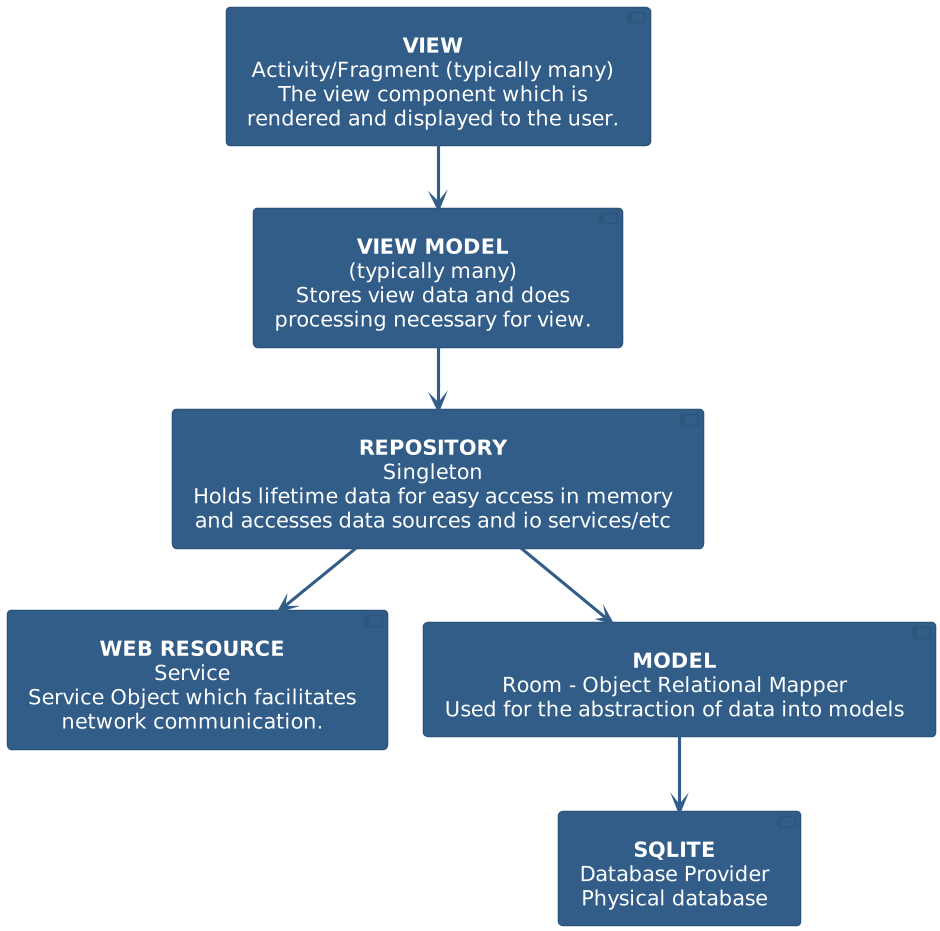
\includegraphics[scale=0.4]{../diag/mvvm_layout.png}
\caption{Android - \Ac{mvvm} Architecture}
\label{fig:mvvm_layout}
\end{figure}

\subsubsection{Android - \ac{di} with Hilt}
Hilt is an android library used for easily implementing \ac{di}.
It has support for common android components.
\cite{noauthor_dependency_nodate}

\subsubsection{Android - Running continuously in the background}
Tracking \ac{app}s need to run continuosly, without forcing the user to keep the \ac{app} view components open.
This can be achieved by implementing the tracking component as a \textit{foreground service}.
In this way, the component runs continuously while allowing the user to use other applications.

Users must also be notified of continuously running services for clarity.
It is therefore required display notifications about the service.
\cite{noauthor_foreground_nodate}

\subsubsection{Android - SQLite database with the Room \ac{orm}}
The Room \ac{orm} library provides a neat database abstraction layer over SQLite useful for modeling data.
SQLite is preferable for android due to its lightweight nature.
\cite{noauthor_save_nodate}

The storage capacity of SQLite is basically unlimited.
Storage capacity is, however, limited to the storage capability of the smartphone running the application.
This makes the use of external storage desirable.

\subsection{\ac{io} Server}
The \ac{io} server is required for relaying logged data from the smartphone application to the central data store. It must be many clients quickly and efficiently.
This server plays a typical server role; In that it must await requests from clients attempting to establish connection for transmitting data.

Implementations for realizing such a server are possible in many programming languages, and almost all top popular programming languages. 
Generally, for performance-critical applications, C and/or C++ are considered most appropriate. \cite{ogala2020comparative}

\subsubsection{Asynchronous \Ac{io}}
Servers (and many other application) are required to run relatively slow operations; that is communicating over networks and writing to disk.
Implementing such functionality synchronously (using blocking calls) leaves functions essentially waiting for data streams to be read, transmitted and written to disk.
This is slow and incapable of handling multiple simultaneous connections.

Asynchronous \ac{io} operations enables other processing to continue before a slow \ac{io} operation has completed.
This is essential for servers which handle many simultaneous connections.
A popular C++ library, \textit{asio} provides asynchronous \ac{io} functionality.
\cite{anggoro2015boost}

\subsection{Database Considerations}
\ac{rdbms}s are commonly used in for data handling.
Typically, for unnormalized complex data, conventional \ac{sql} \ac{rdbms}s prove inefficient at scale, due to the tendency of modern data catalogues lacking in structure.
In addition, relational databases also start to exhibit slower lookup times for immensely large data sets.
The solution to this comes in the form of \ac{nosql} database systems, which are scaleable, efficient and capable for storing large volumes of unnormalized data. \cite{gupta2017nosql} \cite{qader2018comparative} \cite{ongo2018hybrid}

However, due to the completely uniform structure of the data being stored, an \ac{rdbms} would suffice.
Numerous high quality \ac{rdbms}s, such as MySQL, Microsoft SQL, PostgreSQL, and Oracle Database are available, among others. All options offer relatively efficient performance.
\cite{truskowski2020comparison}

A lightweight caching database is necessary on the client-side for the momentary storage of data which has yet to be transmitted to the server. To this end, SQLite offers a popular solution for smartphone applications \cite{bhosale2015sqlite}.

\subsection{Web Application}
The web application will be used by managers to display daily reports highlighting their truckers' behavior throughout their shifts.

The web application may be easily realized by utilizing pre-existing web frameworks, such as Microsoft's ASP.NET Core and Oracle's Java Enterprise Edition (with comparable performance) \cite{kronis2018performance}.

\subsubsection{\Ac{mvc} design pattern for web applications}
\begin{figure}
\centering
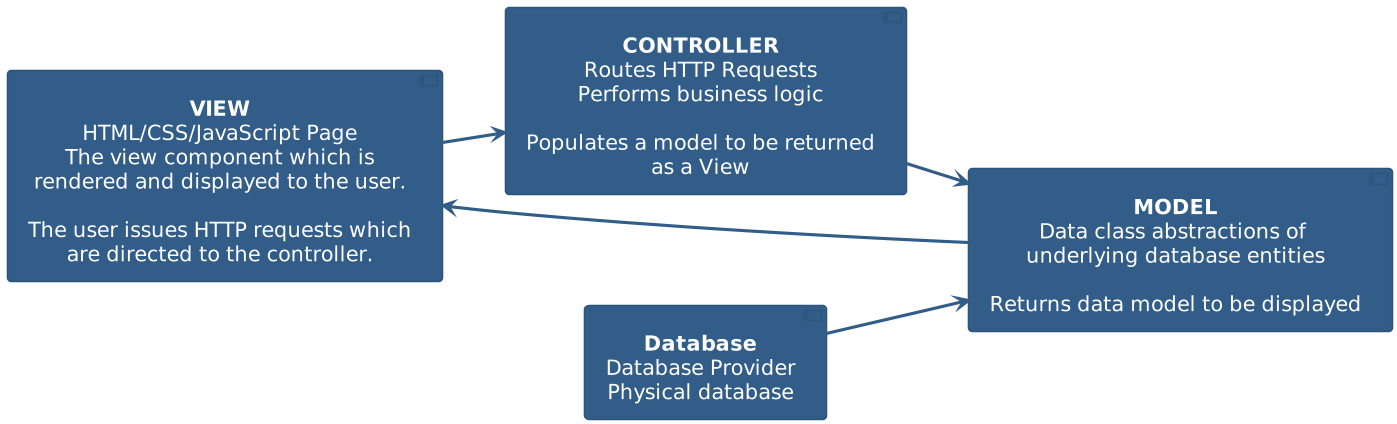
\includegraphics[width=6in]{../diag/mvc_layout.png}
\caption{Web Design Pattern - \ac{mvc}}
\label{fig:mvc_layout}
\end{figure}

A relatively popular design pattern in web development is the \ac{mvc} architecture.
As seen in figure \ref{fig:mvc_layout}, \ac{mvc} attempts to achieve \ac{soc} by separating logic required for viewing, routing and data into separate components.

\subsection{Secure communication with \ac{ssl}}
The use of secure communication over the internet is a modern-day standard.
And due to sensitive location data being transmitted, it is necessary to ensure that logs are adequately encrypted.

The \ac{ssl} protocol is a de facto standard for encrypted communication on the internet.
\Ac{ssl} itself is deprecated, and the current standard for encryption is \ac{tls}.
However, it is common to refer to refer to these related technologies interchangeably, when \ac{tls} is the protocol actually in use. \cite{hickman1995ssl}

\subsection{Serialization and communication protocols}
Facilitating communication between two devices requires both devices to use the same protocol.
Regardless of this protocol, it is necessary for communication to be encrypted, therefore making use of \ac{ssl}.

\subsubsection{\Ac{https}}
\Ac{https} implements the de facto \Ac{http} protocol over the encrypted \ac{ssl} protocol.
\Ac{http} is an application layer protocol which makes use of standard headers carrying a payload under formalized request types, of which \textit{GET} and \textit{POST} are common.
\Ac{https} is commonly used for web services and websites.
\cite{fielding1999hypertext}.

\subsubsection{\Ac{json} and \Ac{xml}}
\Ac{xml} is a strongly-typed text protocol which can be used for serialization.
It follows a tight tagging schema.

\Ac{json} is a fast and simple text protocol for serializing objects carrying data.
Support for arrays makes \ac{json} reliable for the transmission of many logs.
\cite{nurseitov2009comparison}

\pagebreak
